\section{Concept of Entanglement}

Let us define our total Hilbert space as $\mathcal{H}_{\text{total}} = \mathcal{H}_a \otimes \mathcal{H}_b$ (e.g. two quantum bits together $\mathcal{H}_a = \mathbb{C}^2, \mathcal{H}_b = \mathbb{C}^2$).
\begin{definition}
Product state $\ket{\varphi}$ are such that 
\begin{align*} 
	\exists \ket{\varphi_a} \in \mathcal{H}_a, \ket{\varphi_b} \in \mathcal{H}_b 
\end{align*}
such that $\mathcal{H}_{\text{total}} \in \ket{\varphi} = \ket{\varphi_a} \otimes \ket{\varphi_b}$
\end{definition}
What we mean is that a state is a product state if our state $\ket{\varphi}$ can be written as a tensor product between to state from each Hilbert space $\mathcal{H}_a$ and $\mathcal{H}_b$.

\begin{definition}
\important{Entangled states} are states which cannot be written as a tensor product of two state, state that are not product state.
\end{definition} 



\begin{parag}{Example}
    If we take for instance the following state inside $\mathbb{C}^2 \otimes \mathbb{C}^2$:
	\begin{align*} 
		\ket{\varphi}=  \ket{+} \otimes \ket{-} &= \frac{\ket{0} + \ket{1`}}{\sqrt{2}} \otimes \frac{\ket{0} - \ket{1}}{\sqrt{2}}\\
		&= \frac{1}{2}\left(\ket{00} - \ket{01} + \ket{10} - \ket{11}\right)
	\end{align*}
	Here we have that $\ket{\varphi}$ is a product state by construction.\\
	$ $\\
	Let us for instance change a minus sign in our state giving 
	\begin{align*} 
		\ket{\psi} = \frac{1}{2}\left(\ket{00} - \ket{01} + \ket{10} + \ket{11}\right) 
	\end{align*}
	To prove that the state $\ket{\psi}$ is not a product state, we can do the following by contradiction. Assume that our state is entangled, then we know that there exists four coefficients such that 
	\begin{align*} 
		\ket{\psi} = \left(\alpha \ket{0} + \beta \ket{1}\right) \otimes \left(\gamma \ket{0} + \delta \ket{1}\right) 
	\end{align*}
	Here one can just develop our four equalities giving us the following system 
	\begin{align*} 
		\begin{cases}
			\alpha \gamma = \frac{1}{2} \\
			\alpha \delta = - \frac{1}{2}\\
			\beta \gamma = \frac{1}{2}\\
			\beta  \delta = \frac{1}{2}
		\end{cases}  
	\end{align*}
	If we were working with real number, this can be proven fairly easily as the product of the LHS would be positive whereas the RHS would me negative ($-\frac{1}{16}$). But as we are working with complex number one should show it differently, what we need to do here is to make the modulus pop out. To do so, one can just take the conjugate as we have that $\overline{\alpha}\overline{\gamma} = \frac{1}{2}$ and that $\overline{\beta}\overline{\delta} = \frac{1}{2}$. Which when now multiplying everything together gives 
	\begin{align*} 
		\left|\alpha\right|^2\left|\beta\right|^2\left|\gamma\right|^2\left|\delta\right|^2 = - \frac{1}{16} 
	\end{align*}
	Which is a contradiction.
\end{parag}


\subsection{Bell states}
There are four states that plays a special roles in quantum communication and information theory, namely in teleportation, dense coding but also in QKD and many more topics. Those state are the '\textit{maximum entangled}'\\
\begin{parag}{What are those?}
    The bell states form an orthogonal basis of the state of two qbits $\mathbb{C}^2 \otimes \mathbb{C}^2$. Those state are given as 
	\begin{align*} 
		\ket{B_{00}} = \frac{1}{\sqrt{2}} \left(\ket{0}_A \otimes \ket{0}_B + \ket{1}_A \otimes \ket{1}_B\right) \\
		\ket{B_{01}} = \frac{1}{\sqrt{2}} \left(\ket{0}_A \otimes \ket{1}_B + \ket{1}_A \otimes \ket{0}_B\right) \\
		\ket{B_{10}} = \frac{1}{\sqrt{2}} \left(\ket{0}_A \otimes \ket{0}_B - \ket{1}_A \otimes \ket{1}_B\right)\\
		\ket{B_{11}} = \frac{1}{\sqrt{2}}\left(\ket{0}_A \otimes \ket{1}_B - \ket{1}_A \otimes \ket{0}_B\right)
	\end{align*}
	Here, one can show here that those states are entangled.

\end{parag}
\begin{parag}{Computational orthogonal basis}
    Let us also define the computational orthogonal basis of our new space $\mathbb{C}^2 \otimes \mathbb{C}^2$ namely 
	\begin{align*} 
		\ket{0} \otimes \ket{0} &= \begin{pmatrix} 1 \\ 0 \\ 0 \\ 0 \end{pmatrix}  \mathspace \mathspace \ket{0} \otimes \ket{1} = \begin{pmatrix} 0 \\ 1 \\ 0 \\ 0 \end{pmatrix} \\
		\ket{1} \otimes \ket{0} &= \begin{pmatrix} 0 \\ 0 \\ 1 \\ 0 \end{pmatrix}  \mathspace \mathspace\ket{1} \otimes \ket{1} = \begin{pmatrix} 0 \\ 0 \\ 0 \\ 1 \end{pmatrix} 
	\end{align*}
\end{parag}

\begin{parag}{Important property of $\ket{B_{00}}$}
    Let us define the state $\ket{\theta} = \cos \theta \ket{0} + \sin \theta \ket{1}$ which is the polarization state of a photon by $\theta$. Then we can also define the perpendicular  state
	\begin{align*} 
		\ket{\theta_\perp} = -\sin \theta \ket{0} + \cos \theta \ket{1}
	\end{align*}
	\begin{theoreme}
	\begin{align*} 
		\ket{B_{00}}   = \frac{1}{\sqrt{2}}\left(\ket{\theta}_A \otimes \ket{\theta}_B + \ket{\theta_\perp} \otimes \ket{\theta_\perp}_B\right)
	\end{align*}
	\end{theoreme}
	What this implies is that the entanglement here $\ket{B_{00}}$ is angle independent. In Alice's lab, the angle of our state locally is sort of '\textit{random}' but is the \important{same} as the state inside Bob's lab. What we mean here by that which we will see later is that the entropy of our angle in both labs are maximized.
	\begin{subparag}{Remark}
	    The prove for all $\theta$ is left to the reader.
	\end{subparag}

\end{parag}



\subsection{Teleportation}
Assume that we have Alice $A^{\text{earth}}$ on earth which has a photon in a state $\ket{\varphi}_1 = \alpha \ket{0}_1 + \beta \ket{1}_1$ where $\alpha, \beta \in \mathbb{C}$ are unknown.
\begin{parag}{Protocol}
	\begin{center}
	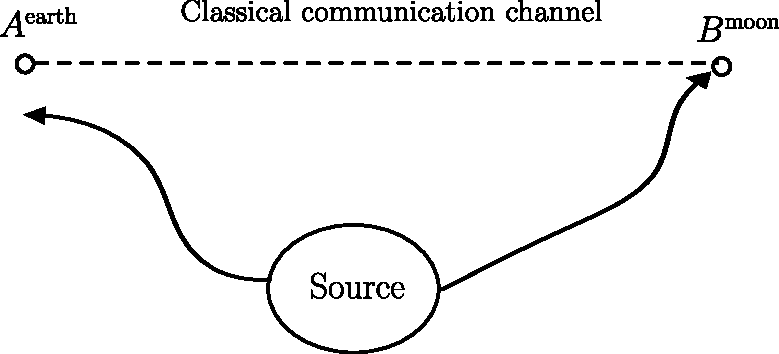
\includegraphics[width=0.6\textwidth]{figures/2026-10-07.pdf}
	\end{center}
	Given our initial state $\ket{\varphi}_1 \otimes \ket{B_{00}}_{23}$ the goal of the protocol is to '\textit{teleport}' the state $\ket{\varphi}$ from $A$ to $B$, $\ket{\varphi}_1 \longrightsquigarrow \ket{\varphi}_3$ where we have the entangled state $\ket{B_{00}}$ being split with one qbit to Alice $\ket{\varphi}_2$ and the other to Bob $\ket{\varphi}_3$ (note that we say separate in the sense that one qbit is at Alice's location and the other at Bob's location and not as two separate states).
	\begin{subparag}{First step}
	    Alice does a local measurement of her two qbits with apparatus that's equivalent to a Bell basis.
	\end{subparag}
	\begin{subparag}{Second step}
	    Alice observes her result, one among $\ket{B_{00}}, \ket{B_{01}}, \ket{B_{10}}, \ket{B_{11}}$ and sends two classical bits of information through the classical channel.
	\end{subparag}
	\begin{subparag}{Third step}
		Bob receives the classical message $ij \in \left\{00, 01, 10, 11\right\}$ and will do a local unitary operation on his qbit. 
		\begin{itemize}
		    \item If he receives $00 \to I_3$
		    \item $01 \to X_3 =  \begin{pmatrix} 0 & 1 \\ 1 & 0 \end{pmatrix} $
		    \item $10 \to Z_3 = \begin{pmatrix} 1 & 0 \\ 0 & -1 \end{pmatrix} $
		    \item $11 \to Z_3X_3 = \begin{pmatrix} 0 & -1 \\ 1 & 0 \end{pmatrix} $
		\end{itemize}
		Then Bob receives exactly $\ket{\varphi}_3 =  \alpha \ket{0}_3 + \beta \ket{1}_3$
	\end{subparag}
\end{parag}
\begin{parag}{Analysis}
    The measurement projects the state of Alice, suppose for the analysis that she get $\ket{B_{01}}$ (the same argument can be done for any other bell states), what this implies is that our state is projected onto $\ket{B_{01}}$ using the following projector
	\begin{align*} 
		\ket{B_{01}}_{12}\bra{B_{01}}_{12}
	\end{align*}
	In Bob's lab nothing has happened which implies that the first operation is a construction using the above projector and the identity applied to our state which gives the following 
	\begin{align*} 
	\left(\ket{B_{01}}_{12}\bra{B_{01}}_{12} \otimes I_3\right)\left(\ket{\varphi}_1 \otimes \ket{B_{00}}_{23}\right) = \ket{B_{01}}_{12} \otimes \underbrace{\bra{B_{01}}_{12} \ket{\phi}_1 \otimes \ket{B_{00}}_{23}}_{\text{state vector for 3 in Bob's lab}} 
	\end{align*}
	As we can see, there is not entanglement now between $2$ and $3$ but $1$ and $2$ are now entangled. Let us now compute the right par of the RHS which gives us 
	\begin{align*} 
		&\frac{1}{\sqrt{2}} \left(\bra{0}_1 \otimes \bra{1}_2 + \bra{1}_1 \otimes \bra{0}_1\right)\left(\alpha \ket{0}_1 + \beta \ket{1}_1\right) \otimes \frac{1}{\sqrt{2}}\left(\ket{0}_2 \otimes \ket{0}_3 + \ket{1}_2 \otimes \ket{1}_3\right)\\
		&= \frac{1}{\sqrt{2}} \left(\alpha \bra{1}_2 + \beta \bra{0}_2\right) \otimes \frac{1}{\sqrt{2}} \left(\ket{0}_2 \otimes \ket{0}_3 + \ket{1}_2 \otimes \ket{1}_3\right) \\
		&= \frac{1}{2}\left(\alpha \ket{1}_3 + \beta \ket{0}_3\right)
	\end{align*}
	But as we didn't normalized after the measurement we should do it now giving us 
	\begin{align*} 
		=  \alpha \ket{1}_3 + \beta \ket{0}_3
	\end{align*}
	Then after this he receives from Alice the two bits $01$ which means that he needs to apply $X_3$ giving us 
	\begin{align*} 
		X\left(\alpha \ket{1}_3 + \beta \ket{0}_3\right) &= \alpha X \ket{1} + \beta X \ket{0}\\
		 &= \alpha \ket{0} + \beta \ket{1} =  \ket{\varphi}_3
	\end{align*}
\end{parag}



\subsection{Dense coding}

\begin{figure}[h!]
\centering
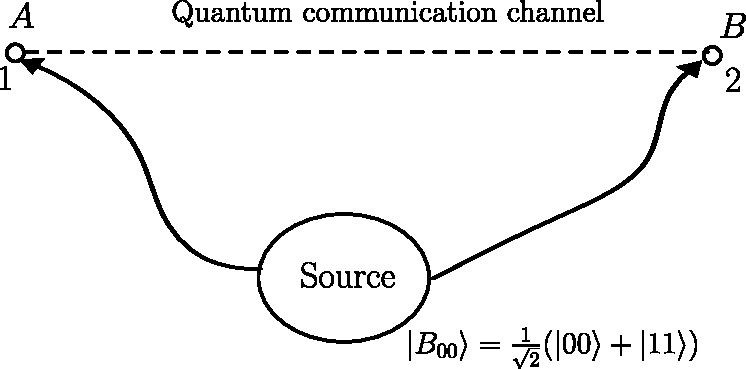
\includegraphics[width=0.6\textwidth]{figures/2026-10-07_1.pdf}
\caption{Dense coding protocol}
\end{figure}
The goal is that Alice transmits two classical bits to Bob using only one qbit.
\begin{parag}{Protocol}
    \begin{itemize}
        If Alice wants to send $00$, A will sends with $I_1$ and send the qbit to Bob $\implies$ Bob receives full EPR pair $\ket{B_{00}}_{\text{Bob}}$
        \item If Alice want to send $01$, Alice will apply $X_1$ and send the qbit to Bob $\implies$ Bob receives $\left(X_1 \otimes I_2\right)\ket{B_{00} = \ket{B_{01}}}_{\text{Bob}}$
        \item If Alice want to send $10$, Alice will apply $Z_1$ and send the qbit to Bob $\implies$ Bob receives $\left(Z_1 \otimes I_2\right)\ket{B_{00} = \ket{B_{10}}}_{\text{Bob}}$
        \item If Alice want to send $11$, Alice will apply $Z_1X_1$ and send the qbit to Bob $\implies$ Bob receives $\left(Z_1X_1 \otimes I_2\right)\ket{B_{00} = \ket{B_{11}}}_{\text{Bob}}$
    \end{itemize}
	Finally, Bob Measure the full pair in the Bell basis which the output will be $\ket{B_{ij}}_{\text{received}}$ Where $ij$ is the bits that Alice sent.
    
\end{parag}

